\begin{figure}
 \centering
  \begin{columns}
  \begin{column}{0.10\textwidth}
   \textbf{(a)}
  \end{column}
  \begin{column}{0.65\textwidth}
    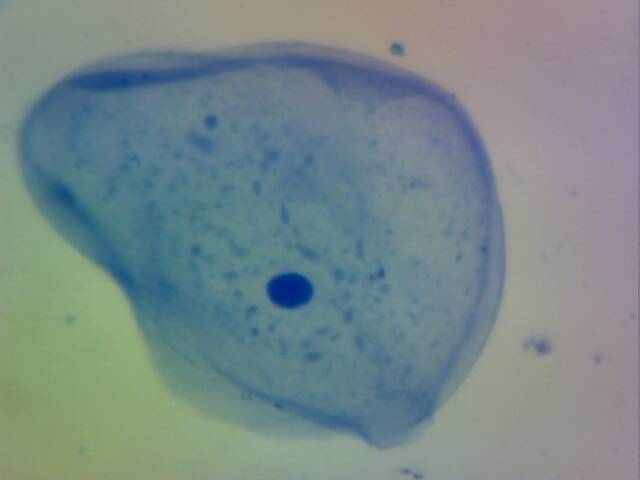
\includegraphics[width=\textwidth]{img/cheek_cell}
  \end{column}
  \begin{column}{0.05\textwidth}
    \cite{clare_and_ben_2017}
  \end{column}
  \end{columns}
  \begin{columns}
  \begin{column}{0.10\textwidth}
   \textbf{(b)}
  \end{column}
  \begin{column}{0.65\textwidth}
    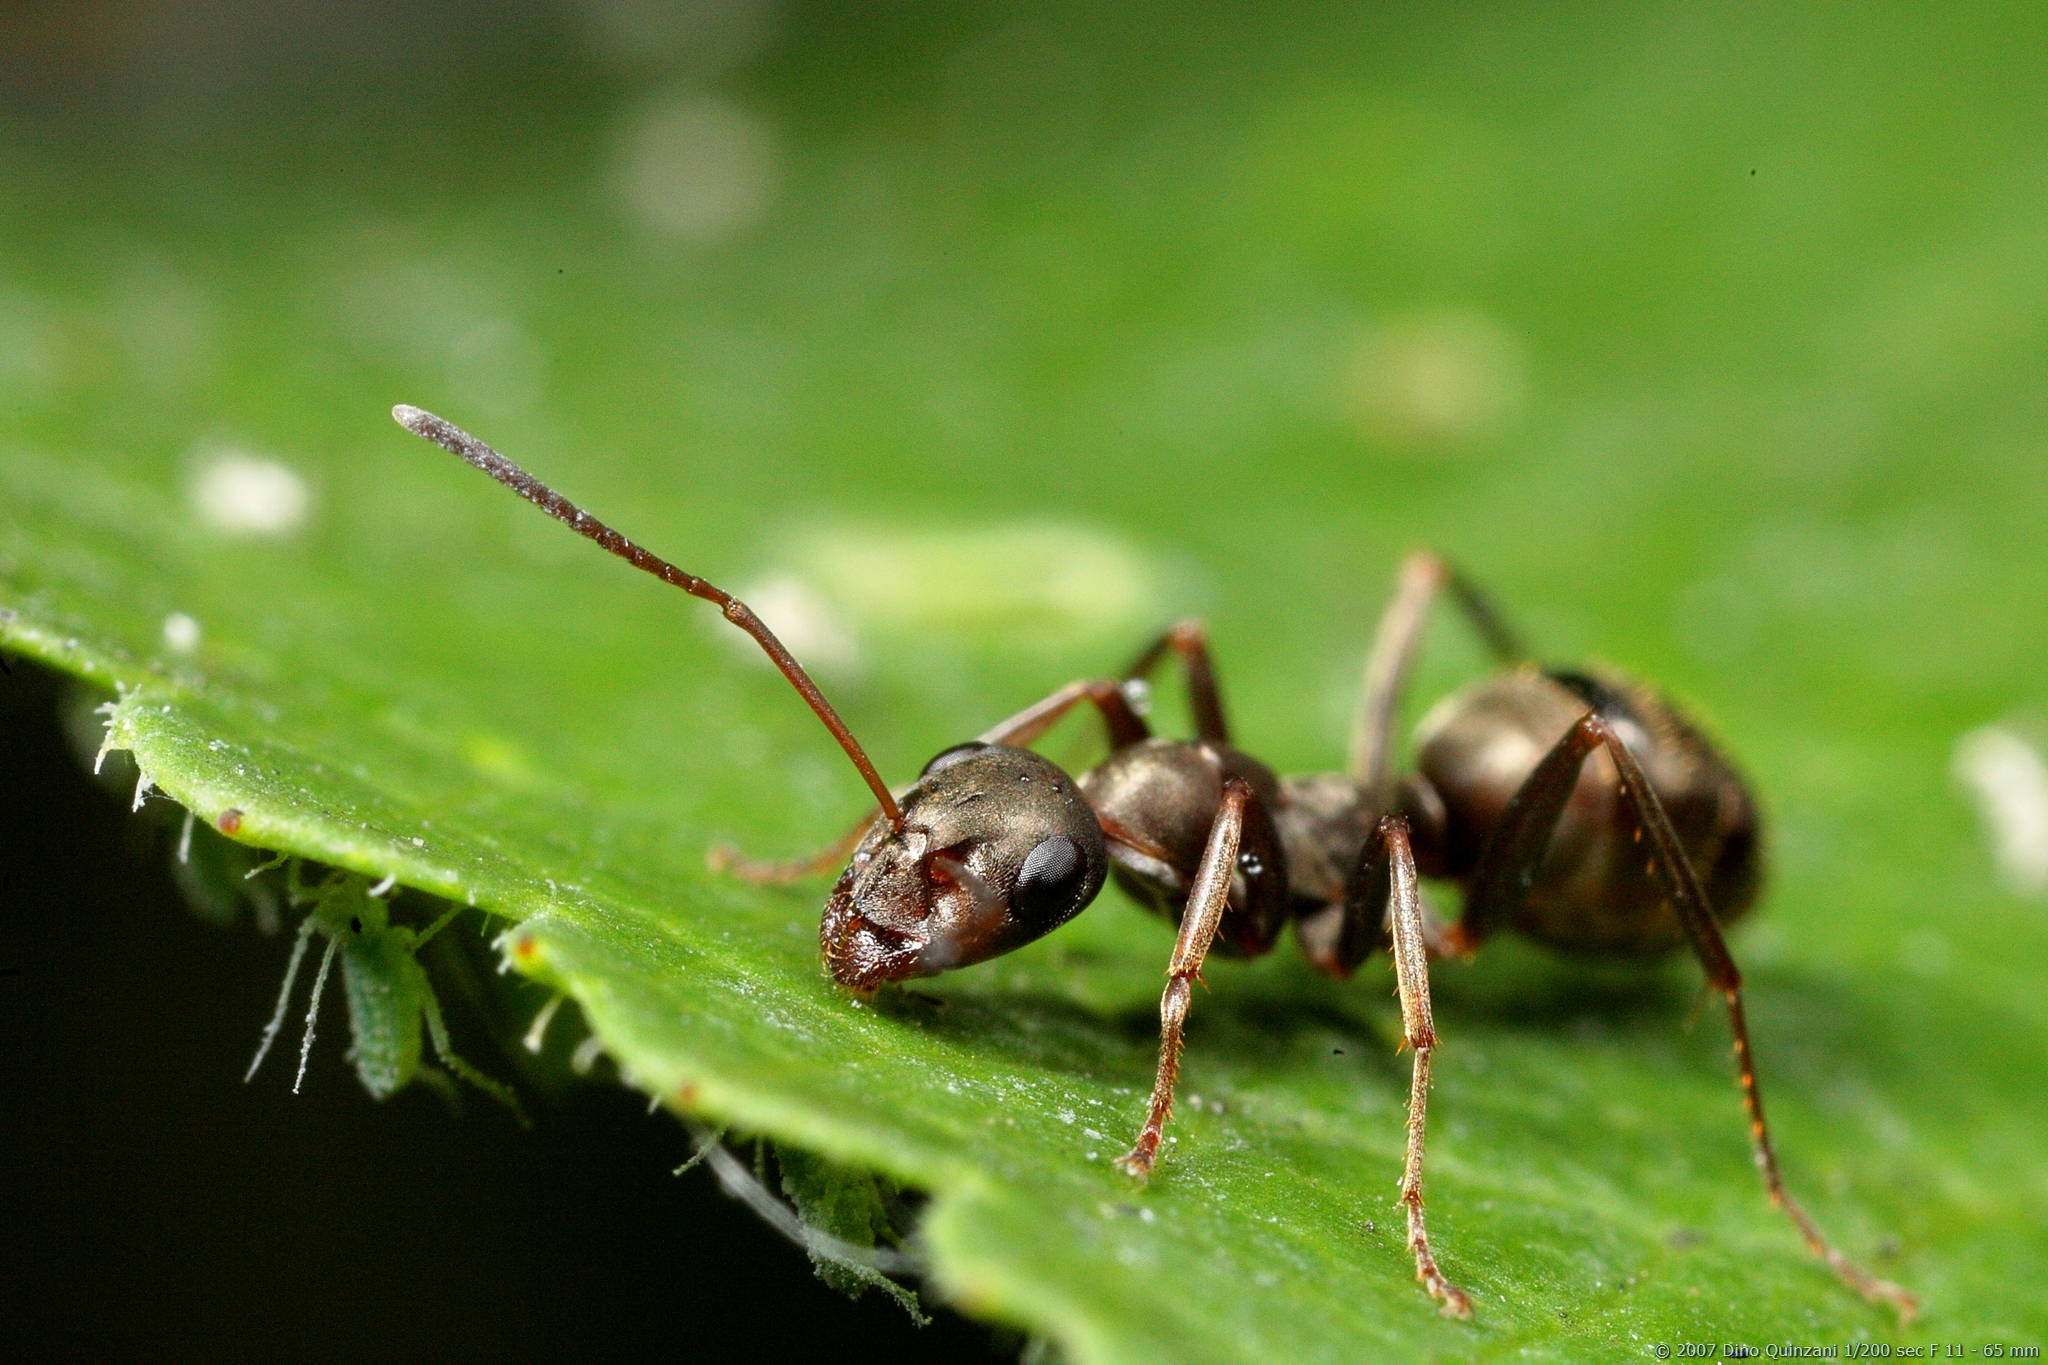
\includegraphics[width=\textwidth]{img/ant}
  \end{column}
  \begin{column}{0.05\textwidth}
    \cite{quinzani_2008}
  \end{column}
  \end{columns}
  \begin{columns}
  \begin{column}{0.10\textwidth}
    \textbf{(c)}
  \end{column}
  \begin{column}{0.65\textwidth}
    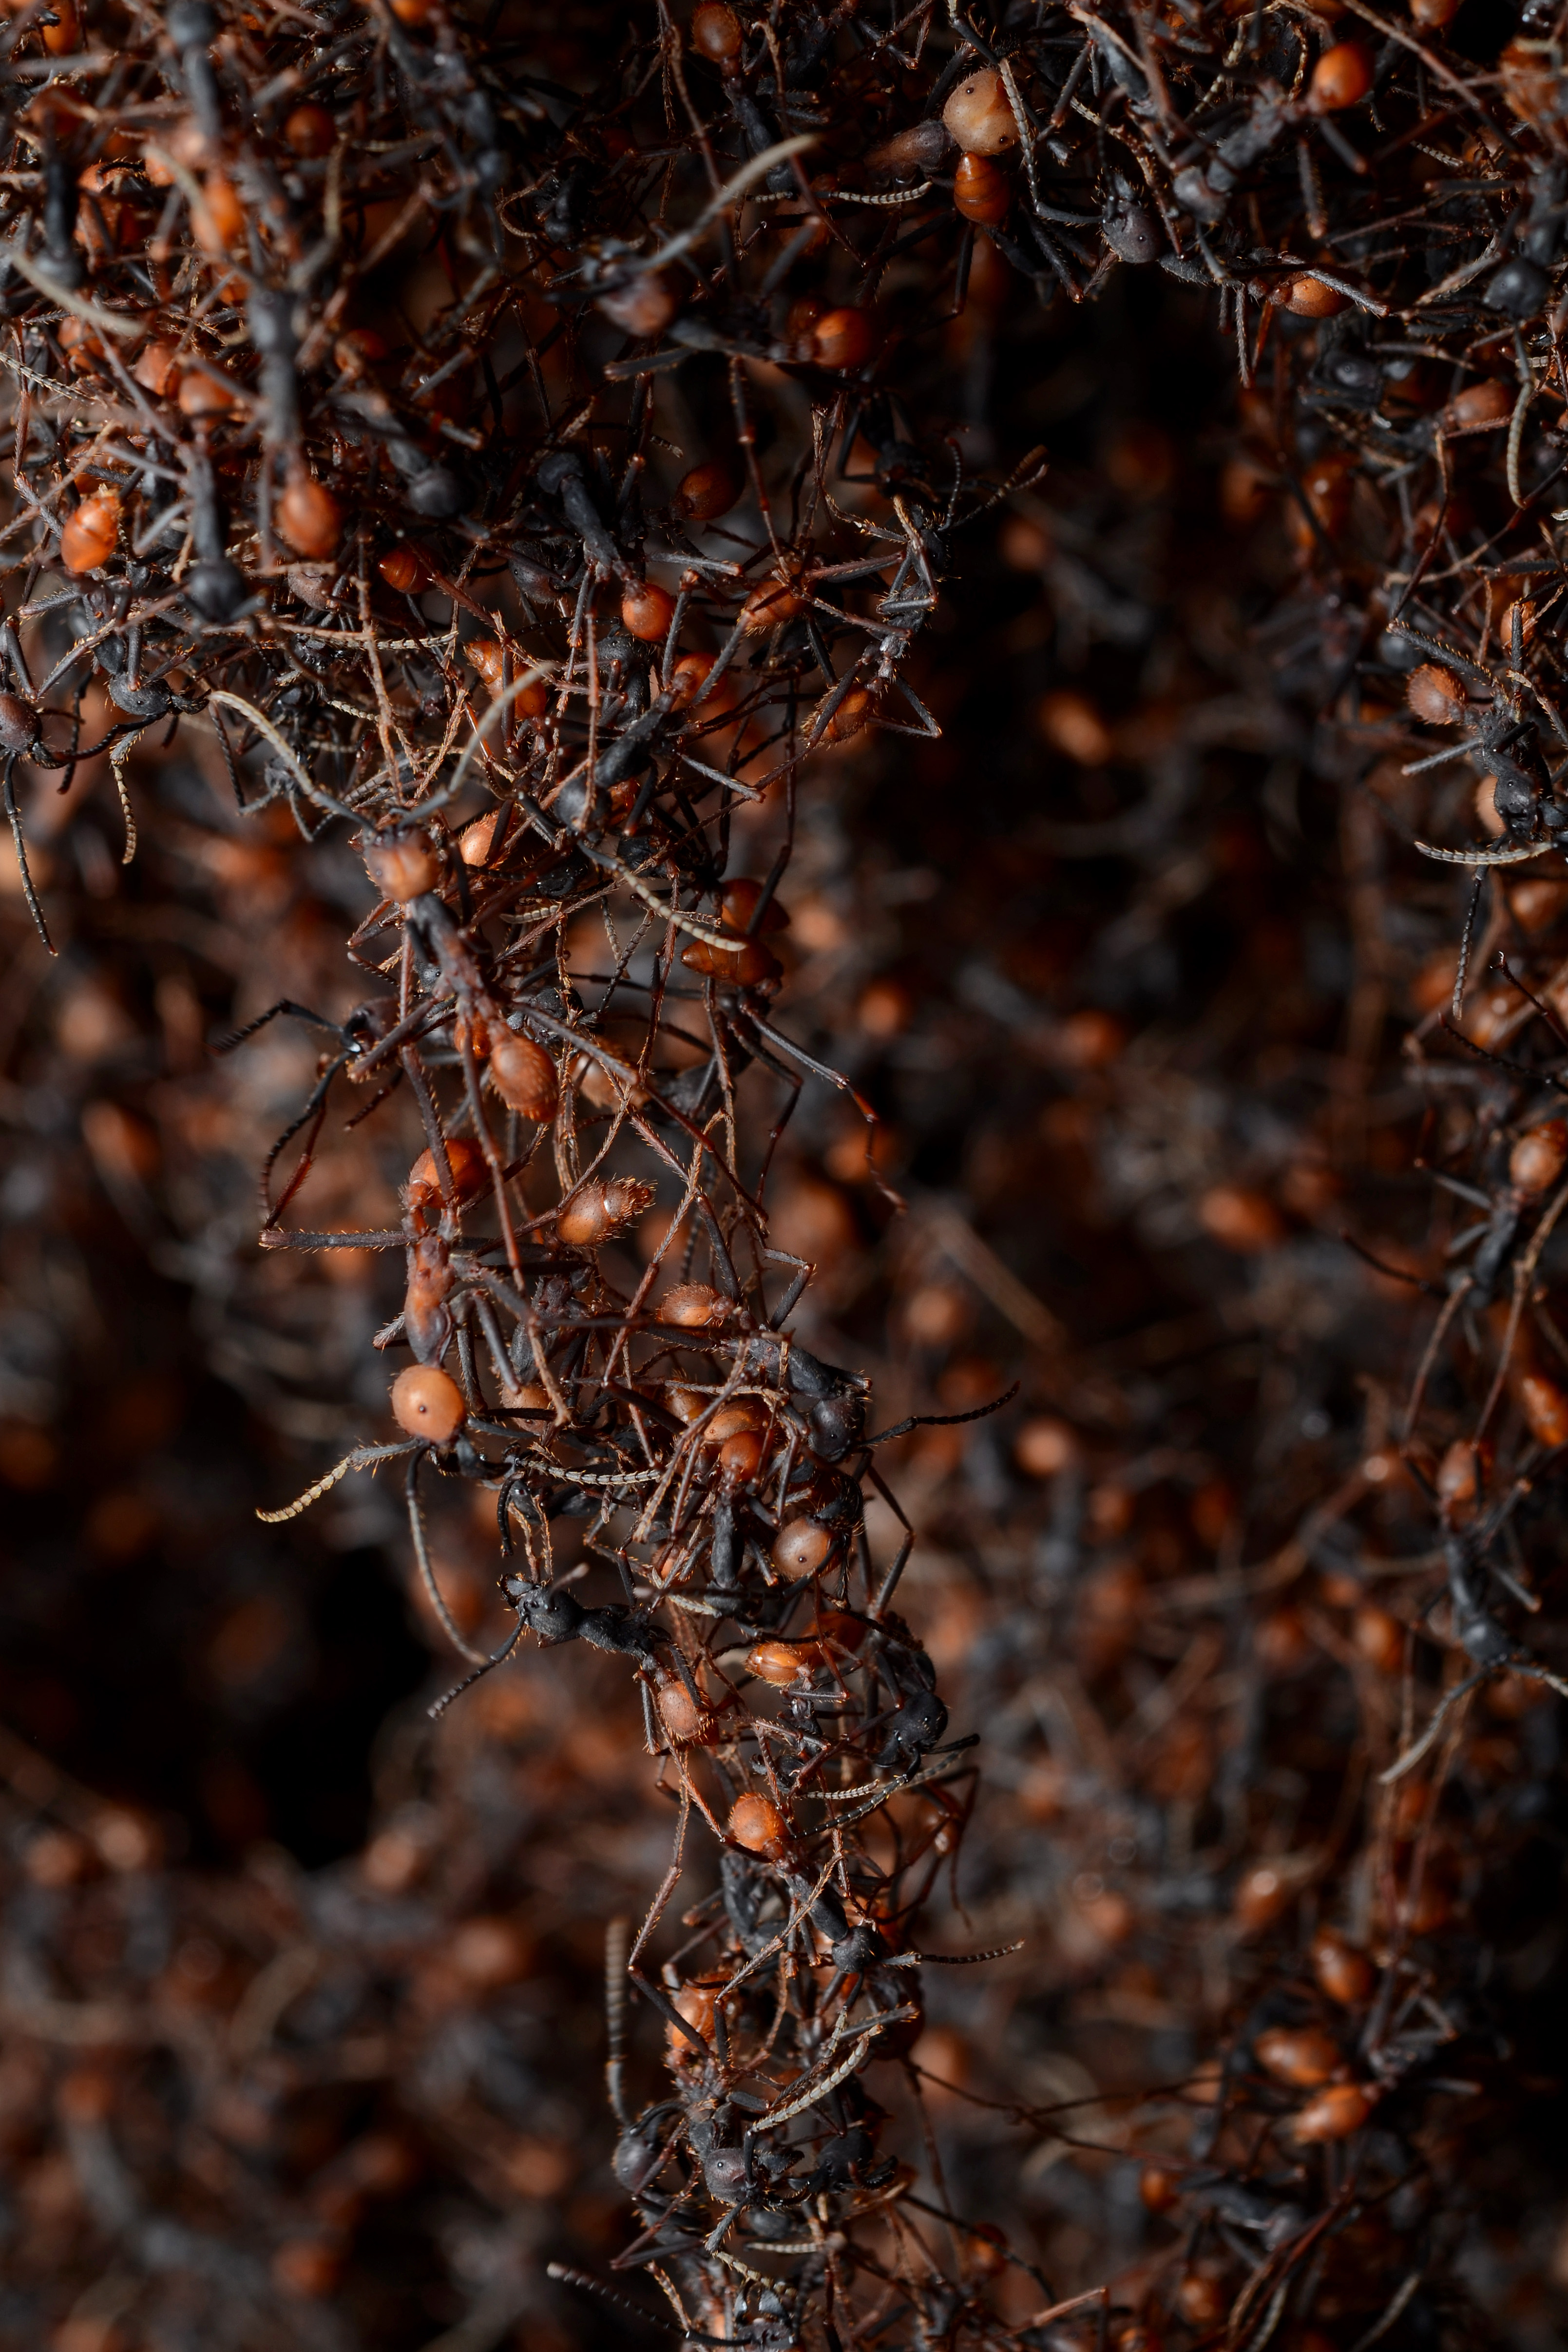
\includegraphics[angle=270,width=\textwidth]{img/ant_bridge}
  \end{column}
  \begin{column}{0.05\textwidth}
    \cite{gallice_2011}
  \end{column}
  \end{columns}
 \caption{
 Example of nested fraternal transitions in individuality where cells (a) unite into multicellular ants (b), which in turn unite into ant colonies (c).
 }
 \label{fig:fraternal}
\end{figure}
